\documentclass[twoside]{book}

% Packages required by doxygen
\usepackage{fixltx2e}
\usepackage{calc}
\usepackage{doxygen}
\usepackage[export]{adjustbox} % also loads graphicx
\usepackage{graphicx}
\usepackage[utf8]{inputenc}
\usepackage{makeidx}
\usepackage{multicol}
\usepackage{multirow}
\PassOptionsToPackage{warn}{textcomp}
\usepackage{textcomp}
\usepackage[nointegrals]{wasysym}
\usepackage[table]{xcolor}

% Font selection
\usepackage[T1]{fontenc}
\usepackage[scaled=.90]{helvet}
\usepackage{courier}
\usepackage{amssymb}
\usepackage{sectsty}
\renewcommand{\familydefault}{\sfdefault}
\allsectionsfont{%
  \fontseries{bc}\selectfont%
  \color{darkgray}%
}
\renewcommand{\DoxyLabelFont}{%
  \fontseries{bc}\selectfont%
  \color{darkgray}%
}
\newcommand{\+}{\discretionary{\mbox{\scriptsize$\hookleftarrow$}}{}{}}

% Page & text layout
\usepackage{geometry}
\geometry{%
  a4paper,%
  top=2.5cm,%
  bottom=2.5cm,%
  left=2.5cm,%
  right=2.5cm%
}
\tolerance=750
\hfuzz=15pt
\hbadness=750
\setlength{\emergencystretch}{15pt}
\setlength{\parindent}{0cm}
\setlength{\parskip}{3ex plus 2ex minus 2ex}
\makeatletter
\renewcommand{\paragraph}{%
  \@startsection{paragraph}{4}{0ex}{-1.0ex}{1.0ex}{%
    \normalfont\normalsize\bfseries\SS@parafont%
  }%
}
\renewcommand{\subparagraph}{%
  \@startsection{subparagraph}{5}{0ex}{-1.0ex}{1.0ex}{%
    \normalfont\normalsize\bfseries\SS@subparafont%
  }%
}
\makeatother

% Headers & footers
\usepackage{fancyhdr}
\pagestyle{fancyplain}
\fancyhead[LE]{\fancyplain{}{\bfseries\thepage}}
\fancyhead[CE]{\fancyplain{}{}}
\fancyhead[RE]{\fancyplain{}{\bfseries\leftmark}}
\fancyhead[LO]{\fancyplain{}{\bfseries\rightmark}}
\fancyhead[CO]{\fancyplain{}{}}
\fancyhead[RO]{\fancyplain{}{\bfseries\thepage}}
\fancyfoot[LE]{\fancyplain{}{}}
\fancyfoot[CE]{\fancyplain{}{}}
\fancyfoot[RE]{\fancyplain{}{\bfseries\scriptsize Generated by Doxygen }}
\fancyfoot[LO]{\fancyplain{}{\bfseries\scriptsize Generated by Doxygen }}
\fancyfoot[CO]{\fancyplain{}{}}
\fancyfoot[RO]{\fancyplain{}{}}
\renewcommand{\footrulewidth}{0.4pt}
\renewcommand{\chaptermark}[1]{%
  \markboth{#1}{}%
}
\renewcommand{\sectionmark}[1]{%
  \markright{\thesection\ #1}%
}

% Indices & bibliography
\usepackage{natbib}
\usepackage[titles]{tocloft}
\setcounter{tocdepth}{3}
\setcounter{secnumdepth}{5}
\makeindex

% Hyperlinks (required, but should be loaded last)
\usepackage{ifpdf}
\ifpdf
  \usepackage[pdftex,pagebackref=true]{hyperref}
\else
  \usepackage[ps2pdf,pagebackref=true]{hyperref}
\fi
\hypersetup{%
  colorlinks=true,%
  linkcolor=blue,%
  citecolor=blue,%
  unicode%
}

% Custom commands
\newcommand{\clearemptydoublepage}{%
  \newpage{\pagestyle{empty}\cleardoublepage}%
}

\usepackage{caption}
\captionsetup{labelsep=space,justification=centering,font={bf},singlelinecheck=off,skip=4pt,position=top}

%===== C O N T E N T S =====

\begin{document}

% Titlepage & ToC
\hypersetup{pageanchor=false,
             bookmarksnumbered=true,
             pdfencoding=unicode
            }
\pagenumbering{roman}
\begin{titlepage}
\vspace*{7cm}
\begin{center}%
{\Large My Project }\\
\vspace*{1cm}
{\large Generated by Doxygen 1.8.11}\\
\end{center}
\end{titlepage}
\clearemptydoublepage
\tableofcontents
\clearemptydoublepage
\pagenumbering{arabic}
\hypersetup{pageanchor=true}

%--- Begin generated contents ---
\chapter{Hierarchical Index}
\section{Class Hierarchy}
This inheritance list is sorted roughly, but not completely, alphabetically\+:\begin{DoxyCompactList}
\item \contentsline{section}{Fruit}{\pageref{classFruit}}{}
\begin{DoxyCompactList}
\item \contentsline{section}{Apple}{\pageref{classApple}}{}
\item \contentsline{section}{Grape}{\pageref{classGrape}}{}
\item \contentsline{section}{Orange}{\pageref{classOrange}}{}
\end{DoxyCompactList}
\item \contentsline{section}{List}{\pageref{classList}}{}
\item \contentsline{section}{List\+:\+:Node}{\pageref{structList_1_1Node}}{}
\end{DoxyCompactList}

\chapter{Class Index}
\section{Class List}
Here are the classes, structs, unions and interfaces with brief descriptions\+:\begin{DoxyCompactList}
\item\contentsline{section}{\hyperlink{structnode}{node} }{\pageref{structnode}}{}
\item\contentsline{section}{\hyperlink{structnode1}{node1} }{\pageref{structnode1}}{}
\item\contentsline{section}{\hyperlink{structnode__info}{node\+\_\+info} }{\pageref{structnode__info}}{}
\end{DoxyCompactList}

\chapter{File Index}
\section{File List}
Here is a list of all files with brief descriptions\+:\begin{DoxyCompactList}
\item\contentsline{section}{\hyperlink{Lab1_8c}{Lab1.\+c} }{\pageref{Lab1_8c}}{}
\end{DoxyCompactList}

\chapter{Class Documentation}
\hypertarget{classCook}{}\section{Cook Class Reference}
\label{classCook}\index{Cook@{Cook}}


Collaboration diagram for Cook\+:\nopagebreak
\begin{figure}[H]
\begin{center}
\leavevmode
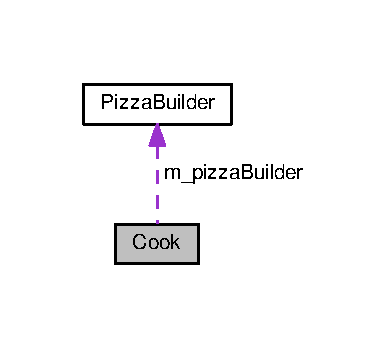
\includegraphics[width=186pt]{classCook__coll__graph}
\end{center}
\end{figure}
\subsection*{Public Member Functions}
\begin{DoxyCompactItemize}
\item 
void \hyperlink{classCook_a980a6342fae6617fc29fdb08101d2372}{open\+Pizza} ()
\item 
void \hyperlink{classCook_a14b38189b02518a8fc89c10529ea59d8}{make\+Pizza} (\hyperlink{classPizzaBuilder}{Pizza\+Builder} $\ast$pb)
\end{DoxyCompactItemize}
\subsection*{Private Attributes}
\begin{DoxyCompactItemize}
\item 
\hyperlink{classPizzaBuilder}{Pizza\+Builder} $\ast$ \hyperlink{classCook_a41e1afd843fef561893f8a4b54972132}{m\+\_\+pizza\+Builder}
\end{DoxyCompactItemize}


\subsection{Member Function Documentation}
\index{Cook@{Cook}!make\+Pizza@{make\+Pizza}}
\index{make\+Pizza@{make\+Pizza}!Cook@{Cook}}
\subsubsection[{\texorpdfstring{make\+Pizza(\+Pizza\+Builder $\ast$pb)}{makePizza(PizzaBuilder *pb)}}]{\setlength{\rightskip}{0pt plus 5cm}void Cook\+::make\+Pizza (
\begin{DoxyParamCaption}
\item[{{\bf Pizza\+Builder} $\ast$}]{pb}
\end{DoxyParamCaption}
)\hspace{0.3cm}{\ttfamily [inline]}}\hypertarget{classCook_a14b38189b02518a8fc89c10529ea59d8}{}\label{classCook_a14b38189b02518a8fc89c10529ea59d8}

\begin{DoxyCode}
104     \{
105         \hyperlink{classCook_a41e1afd843fef561893f8a4b54972132}{m\_pizzaBuilder} = pb;
106         \hyperlink{classCook_a41e1afd843fef561893f8a4b54972132}{m\_pizzaBuilder}->\hyperlink{classPizzaBuilder_ad321d7aede0131b349c6853768ea1735}{createNewPizzaProduct}();
107         \hyperlink{classCook_a41e1afd843fef561893f8a4b54972132}{m\_pizzaBuilder}->\hyperlink{classPizzaBuilder_ab779fb4306ae03b3d82690f5939aaf22}{buildDough}();
108         \hyperlink{classCook_a41e1afd843fef561893f8a4b54972132}{m\_pizzaBuilder}->\hyperlink{classPizzaBuilder_a87b3cc72715e7775c8b36e610e8bb389}{buildSauce}();
109         \hyperlink{classCook_a41e1afd843fef561893f8a4b54972132}{m\_pizzaBuilder}->\hyperlink{classPizzaBuilder_a46ff797a62789eca327a9ffab95b1b23}{buildTopping}();
110     \}
\end{DoxyCode}


Here is the call graph for this function\+:\nopagebreak
\begin{figure}[H]
\begin{center}
\leavevmode
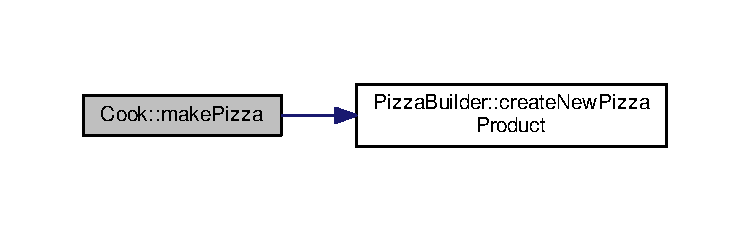
\includegraphics[width=350pt]{classCook_a14b38189b02518a8fc89c10529ea59d8_cgraph}
\end{center}
\end{figure}


\index{Cook@{Cook}!open\+Pizza@{open\+Pizza}}
\index{open\+Pizza@{open\+Pizza}!Cook@{Cook}}
\subsubsection[{\texorpdfstring{open\+Pizza()}{openPizza()}}]{\setlength{\rightskip}{0pt plus 5cm}void Cook\+::open\+Pizza (
\begin{DoxyParamCaption}
{}
\end{DoxyParamCaption}
)\hspace{0.3cm}{\ttfamily [inline]}}\hypertarget{classCook_a980a6342fae6617fc29fdb08101d2372}{}\label{classCook_a980a6342fae6617fc29fdb08101d2372}

\begin{DoxyCode}
100     \{
101         \hyperlink{classCook_a41e1afd843fef561893f8a4b54972132}{m\_pizzaBuilder}->\hyperlink{classPizzaBuilder_a95ce87757351da71ab03f400802a0d1a}{getPizza}()->\hyperlink{classPizza_a7d812bc17133896f57459588988ffd47}{open}();
102     \}
\end{DoxyCode}


\subsection{Member Data Documentation}
\index{Cook@{Cook}!m\+\_\+pizza\+Builder@{m\+\_\+pizza\+Builder}}
\index{m\+\_\+pizza\+Builder@{m\+\_\+pizza\+Builder}!Cook@{Cook}}
\subsubsection[{\texorpdfstring{m\+\_\+pizza\+Builder}{m_pizzaBuilder}}]{\setlength{\rightskip}{0pt plus 5cm}{\bf Pizza\+Builder}$\ast$ Cook\+::m\+\_\+pizza\+Builder\hspace{0.3cm}{\ttfamily [private]}}\hypertarget{classCook_a41e1afd843fef561893f8a4b54972132}{}\label{classCook_a41e1afd843fef561893f8a4b54972132}


The documentation for this class was generated from the following file\+:\begin{DoxyCompactItemize}
\item 
\hyperlink{Builder_8cpp}{Builder.\+cpp}\end{DoxyCompactItemize}

\hypertarget{classHawaiianPizzaBuilder}{}\section{Hawaiian\+Pizza\+Builder Class Reference}
\label{classHawaiianPizzaBuilder}\index{Hawaiian\+Pizza\+Builder@{Hawaiian\+Pizza\+Builder}}


Inheritance diagram for Hawaiian\+Pizza\+Builder\+:\nopagebreak
\begin{figure}[H]
\begin{center}
\leavevmode
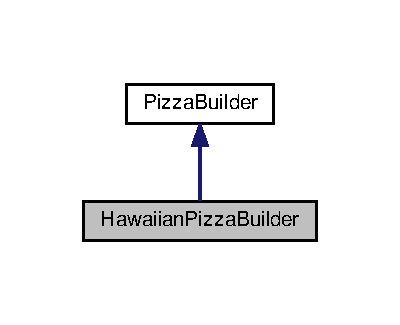
\includegraphics[width=192pt]{classHawaiianPizzaBuilder__inherit__graph}
\end{center}
\end{figure}


Collaboration diagram for Hawaiian\+Pizza\+Builder\+:\nopagebreak
\begin{figure}[H]
\begin{center}
\leavevmode
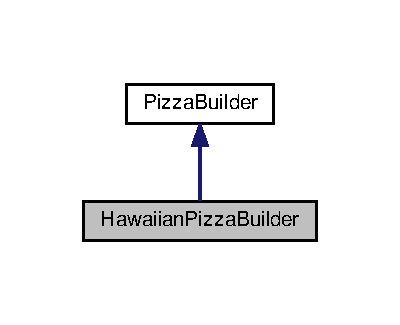
\includegraphics[width=192pt]{classHawaiianPizzaBuilder__coll__graph}
\end{center}
\end{figure}
\subsection*{Public Member Functions}
\begin{DoxyCompactItemize}
\item 
virtual \hyperlink{classHawaiianPizzaBuilder_a621c6b7e508a206a5f85cea4e73fe747}{$\sim$\+Hawaiian\+Pizza\+Builder} ()
\item 
virtual void \hyperlink{classHawaiianPizzaBuilder_a0eddc6f115d76c24a9adfb86dc31a7cc}{build\+Dough} ()
\item 
virtual void \hyperlink{classHawaiianPizzaBuilder_abcfc366ad0ffcec8e93e19807b8eef18}{build\+Sauce} ()
\item 
virtual void \hyperlink{classHawaiianPizzaBuilder_af069af5d54a18d099a6ea6a4382fb42b}{build\+Topping} ()
\end{DoxyCompactItemize}
\subsection*{Additional Inherited Members}


\subsection{Constructor \& Destructor Documentation}
\index{Hawaiian\+Pizza\+Builder@{Hawaiian\+Pizza\+Builder}!````~Hawaiian\+Pizza\+Builder@{$\sim$\+Hawaiian\+Pizza\+Builder}}
\index{````~Hawaiian\+Pizza\+Builder@{$\sim$\+Hawaiian\+Pizza\+Builder}!Hawaiian\+Pizza\+Builder@{Hawaiian\+Pizza\+Builder}}
\subsubsection[{\texorpdfstring{$\sim$\+Hawaiian\+Pizza\+Builder()}{~HawaiianPizzaBuilder()}}]{\setlength{\rightskip}{0pt plus 5cm}virtual Hawaiian\+Pizza\+Builder\+::$\sim$\+Hawaiian\+Pizza\+Builder (
\begin{DoxyParamCaption}
{}
\end{DoxyParamCaption}
)\hspace{0.3cm}{\ttfamily [inline]}, {\ttfamily [virtual]}}\hypertarget{classHawaiianPizzaBuilder_a621c6b7e508a206a5f85cea4e73fe747}{}\label{classHawaiianPizzaBuilder_a621c6b7e508a206a5f85cea4e73fe747}

\begin{DoxyCode}
59 \{\};
\end{DoxyCode}


\subsection{Member Function Documentation}
\index{Hawaiian\+Pizza\+Builder@{Hawaiian\+Pizza\+Builder}!build\+Dough@{build\+Dough}}
\index{build\+Dough@{build\+Dough}!Hawaiian\+Pizza\+Builder@{Hawaiian\+Pizza\+Builder}}
\subsubsection[{\texorpdfstring{build\+Dough()}{buildDough()}}]{\setlength{\rightskip}{0pt plus 5cm}virtual void Hawaiian\+Pizza\+Builder\+::build\+Dough (
\begin{DoxyParamCaption}
{}
\end{DoxyParamCaption}
)\hspace{0.3cm}{\ttfamily [inline]}, {\ttfamily [virtual]}}\hypertarget{classHawaiianPizzaBuilder_a0eddc6f115d76c24a9adfb86dc31a7cc}{}\label{classHawaiianPizzaBuilder_a0eddc6f115d76c24a9adfb86dc31a7cc}


Implements \hyperlink{classPizzaBuilder_ab779fb4306ae03b3d82690f5939aaf22}{Pizza\+Builder}.


\begin{DoxyCode}
62     \{
63         \hyperlink{classPizzaBuilder_a76a40bb3d715332acfaeea121e03d9b1}{m\_pizza}->setDough(\textcolor{stringliteral}{"cross"});
64     \}
\end{DoxyCode}
\index{Hawaiian\+Pizza\+Builder@{Hawaiian\+Pizza\+Builder}!build\+Sauce@{build\+Sauce}}
\index{build\+Sauce@{build\+Sauce}!Hawaiian\+Pizza\+Builder@{Hawaiian\+Pizza\+Builder}}
\subsubsection[{\texorpdfstring{build\+Sauce()}{buildSauce()}}]{\setlength{\rightskip}{0pt plus 5cm}virtual void Hawaiian\+Pizza\+Builder\+::build\+Sauce (
\begin{DoxyParamCaption}
{}
\end{DoxyParamCaption}
)\hspace{0.3cm}{\ttfamily [inline]}, {\ttfamily [virtual]}}\hypertarget{classHawaiianPizzaBuilder_abcfc366ad0ffcec8e93e19807b8eef18}{}\label{classHawaiianPizzaBuilder_abcfc366ad0ffcec8e93e19807b8eef18}


Implements \hyperlink{classPizzaBuilder_a87b3cc72715e7775c8b36e610e8bb389}{Pizza\+Builder}.


\begin{DoxyCode}
66     \{
67         \hyperlink{classPizzaBuilder_a76a40bb3d715332acfaeea121e03d9b1}{m\_pizza}->setSauce(\textcolor{stringliteral}{"mild"});
68     \}
\end{DoxyCode}
\index{Hawaiian\+Pizza\+Builder@{Hawaiian\+Pizza\+Builder}!build\+Topping@{build\+Topping}}
\index{build\+Topping@{build\+Topping}!Hawaiian\+Pizza\+Builder@{Hawaiian\+Pizza\+Builder}}
\subsubsection[{\texorpdfstring{build\+Topping()}{buildTopping()}}]{\setlength{\rightskip}{0pt plus 5cm}virtual void Hawaiian\+Pizza\+Builder\+::build\+Topping (
\begin{DoxyParamCaption}
{}
\end{DoxyParamCaption}
)\hspace{0.3cm}{\ttfamily [inline]}, {\ttfamily [virtual]}}\hypertarget{classHawaiianPizzaBuilder_af069af5d54a18d099a6ea6a4382fb42b}{}\label{classHawaiianPizzaBuilder_af069af5d54a18d099a6ea6a4382fb42b}


Implements \hyperlink{classPizzaBuilder_a46ff797a62789eca327a9ffab95b1b23}{Pizza\+Builder}.


\begin{DoxyCode}
70     \{
71         \hyperlink{classPizzaBuilder_a76a40bb3d715332acfaeea121e03d9b1}{m\_pizza}->setTopping(\textcolor{stringliteral}{"ham+pineapple"});
72     \}
\end{DoxyCode}


The documentation for this class was generated from the following file\+:\begin{DoxyCompactItemize}
\item 
\hyperlink{Builder_8cpp}{Builder.\+cpp}\end{DoxyCompactItemize}

\hypertarget{classPizza}{}\section{Pizza Class Reference}
\label{classPizza}\index{Pizza@{Pizza}}


Inheritance diagram for Pizza\+:
\nopagebreak
\begin{figure}[H]
\begin{center}
\leavevmode
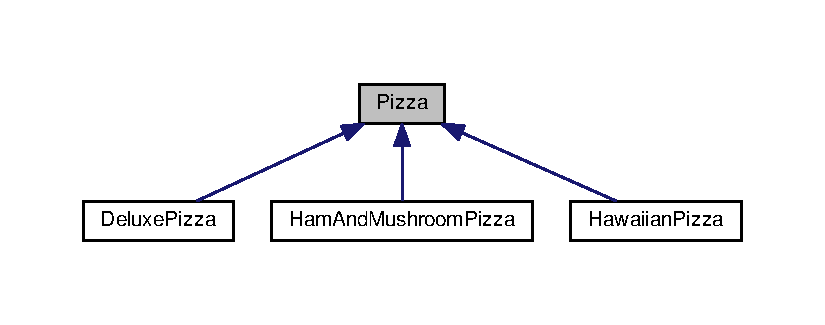
\includegraphics[width=350pt]{classPizza__inherit__graph}
\end{center}
\end{figure}
\subsection*{Public Member Functions}
\begin{DoxyCompactItemize}
\item 
virtual int \hyperlink{classPizza_aa9c7966d23241bfa79efe9f7d9f45408}{get\+Price} () const =0
\item 
virtual \hyperlink{classPizza_a28affbd9b37a895e49aea25360a36a2c}{$\sim$\+Pizza} ()
\end{DoxyCompactItemize}


\subsection{Constructor \& Destructor Documentation}
\index{Pizza@{Pizza}!````~Pizza@{$\sim$\+Pizza}}
\index{````~Pizza@{$\sim$\+Pizza}!Pizza@{Pizza}}
\subsubsection[{\texorpdfstring{$\sim$\+Pizza()}{~Pizza()}}]{\setlength{\rightskip}{0pt plus 5cm}virtual Pizza\+::$\sim$\+Pizza (
\begin{DoxyParamCaption}
{}
\end{DoxyParamCaption}
)\hspace{0.3cm}{\ttfamily [inline]}, {\ttfamily [virtual]}}\hypertarget{classPizza_a28affbd9b37a895e49aea25360a36a2c}{}\label{classPizza_a28affbd9b37a895e49aea25360a36a2c}

\begin{DoxyCode}
9 \{\};  \textcolor{comment}{/* without this, no destructor for derived Pizza's will be called. */}
\end{DoxyCode}


\subsection{Member Function Documentation}
\index{Pizza@{Pizza}!get\+Price@{get\+Price}}
\index{get\+Price@{get\+Price}!Pizza@{Pizza}}
\subsubsection[{\texorpdfstring{get\+Price() const =0}{getPrice() const =0}}]{\setlength{\rightskip}{0pt plus 5cm}virtual int Pizza\+::get\+Price (
\begin{DoxyParamCaption}
{}
\end{DoxyParamCaption}
) const\hspace{0.3cm}{\ttfamily [pure virtual]}}\hypertarget{classPizza_aa9c7966d23241bfa79efe9f7d9f45408}{}\label{classPizza_aa9c7966d23241bfa79efe9f7d9f45408}


Implemented in \hyperlink{classHawaiianPizza_a04efac994727eeb9d772ce9b6654d4f7}{Hawaiian\+Pizza}, \hyperlink{classDeluxePizza_af66f2ac20b82113fc5507a83b63f713c}{Deluxe\+Pizza}, and \hyperlink{classHamAndMushroomPizza_a90a3473504de97256e1b46d7ab60eebb}{Ham\+And\+Mushroom\+Pizza}.



The documentation for this class was generated from the following file\+:\begin{DoxyCompactItemize}
\item 
\hyperlink{Factory_8cpp}{Factory.\+cpp}\end{DoxyCompactItemize}

\hypertarget{classPizzaBuilder}{}\section{Pizza\+Builder Class Reference}
\label{classPizzaBuilder}\index{Pizza\+Builder@{Pizza\+Builder}}


Inheritance diagram for Pizza\+Builder\+:\nopagebreak
\begin{figure}[H]
\begin{center}
\leavevmode
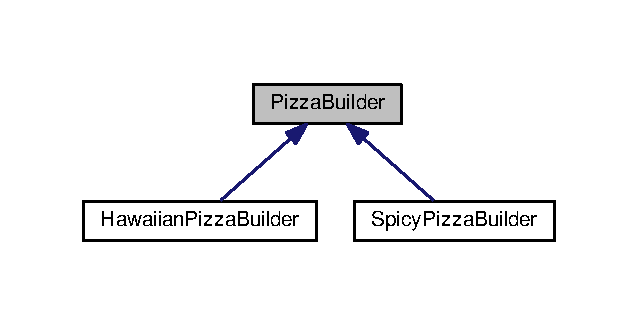
\includegraphics[width=306pt]{classPizzaBuilder__inherit__graph}
\end{center}
\end{figure}
\subsection*{Public Member Functions}
\begin{DoxyCompactItemize}
\item 
virtual \hyperlink{classPizzaBuilder_a424dc27395e06a4c38beca703c91c258}{$\sim$\+Pizza\+Builder} ()
\item 
\hyperlink{classPizza}{Pizza} $\ast$ \hyperlink{classPizzaBuilder_a95ce87757351da71ab03f400802a0d1a}{get\+Pizza} ()
\item 
void \hyperlink{classPizzaBuilder_ad321d7aede0131b349c6853768ea1735}{create\+New\+Pizza\+Product} ()
\item 
virtual void \hyperlink{classPizzaBuilder_ab779fb4306ae03b3d82690f5939aaf22}{build\+Dough} ()=0
\item 
virtual void \hyperlink{classPizzaBuilder_a87b3cc72715e7775c8b36e610e8bb389}{build\+Sauce} ()=0
\item 
virtual void \hyperlink{classPizzaBuilder_a46ff797a62789eca327a9ffab95b1b23}{build\+Topping} ()=0
\end{DoxyCompactItemize}
\subsection*{Protected Attributes}
\begin{DoxyCompactItemize}
\item 
unique\+\_\+ptr$<$ \hyperlink{classPizza}{Pizza} $>$ \hyperlink{classPizzaBuilder_a76a40bb3d715332acfaeea121e03d9b1}{m\+\_\+pizza}
\end{DoxyCompactItemize}


\subsection{Constructor \& Destructor Documentation}
\index{Pizza\+Builder@{Pizza\+Builder}!````~Pizza\+Builder@{$\sim$\+Pizza\+Builder}}
\index{````~Pizza\+Builder@{$\sim$\+Pizza\+Builder}!Pizza\+Builder@{Pizza\+Builder}}
\subsubsection[{\texorpdfstring{$\sim$\+Pizza\+Builder()}{~PizzaBuilder()}}]{\setlength{\rightskip}{0pt plus 5cm}virtual Pizza\+Builder\+::$\sim$\+Pizza\+Builder (
\begin{DoxyParamCaption}
{}
\end{DoxyParamCaption}
)\hspace{0.3cm}{\ttfamily [inline]}, {\ttfamily [virtual]}}\hypertarget{classPizzaBuilder_a424dc27395e06a4c38beca703c91c258}{}\label{classPizzaBuilder_a424dc27395e06a4c38beca703c91c258}

\begin{DoxyCode}
37 \{\};
\end{DoxyCode}


\subsection{Member Function Documentation}
\index{Pizza\+Builder@{Pizza\+Builder}!build\+Dough@{build\+Dough}}
\index{build\+Dough@{build\+Dough}!Pizza\+Builder@{Pizza\+Builder}}
\subsubsection[{\texorpdfstring{build\+Dough()=0}{buildDough()=0}}]{\setlength{\rightskip}{0pt plus 5cm}virtual void Pizza\+Builder\+::build\+Dough (
\begin{DoxyParamCaption}
{}
\end{DoxyParamCaption}
)\hspace{0.3cm}{\ttfamily [pure virtual]}}\hypertarget{classPizzaBuilder_ab779fb4306ae03b3d82690f5939aaf22}{}\label{classPizzaBuilder_ab779fb4306ae03b3d82690f5939aaf22}


Implemented in \hyperlink{classSpicyPizzaBuilder_a31a9b83aff106bf255cdd7b07428cc8f}{Spicy\+Pizza\+Builder}, and \hyperlink{classHawaiianPizzaBuilder_a0eddc6f115d76c24a9adfb86dc31a7cc}{Hawaiian\+Pizza\+Builder}.

\index{Pizza\+Builder@{Pizza\+Builder}!build\+Sauce@{build\+Sauce}}
\index{build\+Sauce@{build\+Sauce}!Pizza\+Builder@{Pizza\+Builder}}
\subsubsection[{\texorpdfstring{build\+Sauce()=0}{buildSauce()=0}}]{\setlength{\rightskip}{0pt plus 5cm}virtual void Pizza\+Builder\+::build\+Sauce (
\begin{DoxyParamCaption}
{}
\end{DoxyParamCaption}
)\hspace{0.3cm}{\ttfamily [pure virtual]}}\hypertarget{classPizzaBuilder_a87b3cc72715e7775c8b36e610e8bb389}{}\label{classPizzaBuilder_a87b3cc72715e7775c8b36e610e8bb389}


Implemented in \hyperlink{classSpicyPizzaBuilder_a74a4d62a67d118b8bbe94721847f38b4}{Spicy\+Pizza\+Builder}, and \hyperlink{classHawaiianPizzaBuilder_abcfc366ad0ffcec8e93e19807b8eef18}{Hawaiian\+Pizza\+Builder}.

\index{Pizza\+Builder@{Pizza\+Builder}!build\+Topping@{build\+Topping}}
\index{build\+Topping@{build\+Topping}!Pizza\+Builder@{Pizza\+Builder}}
\subsubsection[{\texorpdfstring{build\+Topping()=0}{buildTopping()=0}}]{\setlength{\rightskip}{0pt plus 5cm}virtual void Pizza\+Builder\+::build\+Topping (
\begin{DoxyParamCaption}
{}
\end{DoxyParamCaption}
)\hspace{0.3cm}{\ttfamily [pure virtual]}}\hypertarget{classPizzaBuilder_a46ff797a62789eca327a9ffab95b1b23}{}\label{classPizzaBuilder_a46ff797a62789eca327a9ffab95b1b23}


Implemented in \hyperlink{classSpicyPizzaBuilder_a18fccc77e058f373deb851d61074df5b}{Spicy\+Pizza\+Builder}, and \hyperlink{classHawaiianPizzaBuilder_af069af5d54a18d099a6ea6a4382fb42b}{Hawaiian\+Pizza\+Builder}.

\index{Pizza\+Builder@{Pizza\+Builder}!create\+New\+Pizza\+Product@{create\+New\+Pizza\+Product}}
\index{create\+New\+Pizza\+Product@{create\+New\+Pizza\+Product}!Pizza\+Builder@{Pizza\+Builder}}
\subsubsection[{\texorpdfstring{create\+New\+Pizza\+Product()}{createNewPizzaProduct()}}]{\setlength{\rightskip}{0pt plus 5cm}void Pizza\+Builder\+::create\+New\+Pizza\+Product (
\begin{DoxyParamCaption}
{}
\end{DoxyParamCaption}
)\hspace{0.3cm}{\ttfamily [inline]}}\hypertarget{classPizzaBuilder_ad321d7aede0131b349c6853768ea1735}{}\label{classPizzaBuilder_ad321d7aede0131b349c6853768ea1735}

\begin{DoxyCode}
44     \{
45         \hyperlink{classPizzaBuilder_a76a40bb3d715332acfaeea121e03d9b1}{m\_pizza} = make\_unique<Pizza>();
46     \}
\end{DoxyCode}
\index{Pizza\+Builder@{Pizza\+Builder}!get\+Pizza@{get\+Pizza}}
\index{get\+Pizza@{get\+Pizza}!Pizza\+Builder@{Pizza\+Builder}}
\subsubsection[{\texorpdfstring{get\+Pizza()}{getPizza()}}]{\setlength{\rightskip}{0pt plus 5cm}{\bf Pizza}$\ast$ Pizza\+Builder\+::get\+Pizza (
\begin{DoxyParamCaption}
{}
\end{DoxyParamCaption}
)\hspace{0.3cm}{\ttfamily [inline]}}\hypertarget{classPizzaBuilder_a95ce87757351da71ab03f400802a0d1a}{}\label{classPizzaBuilder_a95ce87757351da71ab03f400802a0d1a}

\begin{DoxyCode}
40     \{
41         \textcolor{keywordflow}{return} \hyperlink{classPizzaBuilder_a76a40bb3d715332acfaeea121e03d9b1}{m\_pizza}.release();
42     \}
\end{DoxyCode}


\subsection{Member Data Documentation}
\index{Pizza\+Builder@{Pizza\+Builder}!m\+\_\+pizza@{m\+\_\+pizza}}
\index{m\+\_\+pizza@{m\+\_\+pizza}!Pizza\+Builder@{Pizza\+Builder}}
\subsubsection[{\texorpdfstring{m\+\_\+pizza}{m_pizza}}]{\setlength{\rightskip}{0pt plus 5cm}unique\+\_\+ptr$<${\bf Pizza}$>$ Pizza\+Builder\+::m\+\_\+pizza\hspace{0.3cm}{\ttfamily [protected]}}\hypertarget{classPizzaBuilder_a76a40bb3d715332acfaeea121e03d9b1}{}\label{classPizzaBuilder_a76a40bb3d715332acfaeea121e03d9b1}


The documentation for this class was generated from the following file\+:\begin{DoxyCompactItemize}
\item 
\hyperlink{Builder_8cpp}{Builder.\+cpp}\end{DoxyCompactItemize}

\hypertarget{classSpicyPizzaBuilder}{}\section{Spicy\+Pizza\+Builder Class Reference}
\label{classSpicyPizzaBuilder}\index{Spicy\+Pizza\+Builder@{Spicy\+Pizza\+Builder}}


Inheritance diagram for Spicy\+Pizza\+Builder\+:\nopagebreak
\begin{figure}[H]
\begin{center}
\leavevmode
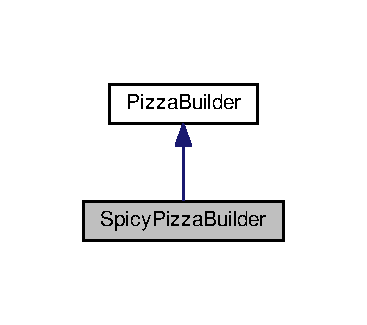
\includegraphics[width=176pt]{classSpicyPizzaBuilder__inherit__graph}
\end{center}
\end{figure}


Collaboration diagram for Spicy\+Pizza\+Builder\+:\nopagebreak
\begin{figure}[H]
\begin{center}
\leavevmode
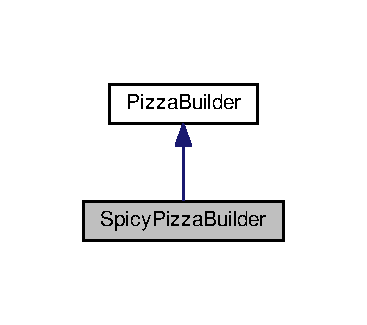
\includegraphics[width=176pt]{classSpicyPizzaBuilder__coll__graph}
\end{center}
\end{figure}
\subsection*{Public Member Functions}
\begin{DoxyCompactItemize}
\item 
virtual \hyperlink{classSpicyPizzaBuilder_ada134c577c76bbe33589074d1eca989b}{$\sim$\+Spicy\+Pizza\+Builder} ()
\item 
virtual void \hyperlink{classSpicyPizzaBuilder_a31a9b83aff106bf255cdd7b07428cc8f}{build\+Dough} ()
\item 
virtual void \hyperlink{classSpicyPizzaBuilder_a74a4d62a67d118b8bbe94721847f38b4}{build\+Sauce} ()
\item 
virtual void \hyperlink{classSpicyPizzaBuilder_a18fccc77e058f373deb851d61074df5b}{build\+Topping} ()
\end{DoxyCompactItemize}
\subsection*{Additional Inherited Members}


\subsection{Constructor \& Destructor Documentation}
\index{Spicy\+Pizza\+Builder@{Spicy\+Pizza\+Builder}!````~Spicy\+Pizza\+Builder@{$\sim$\+Spicy\+Pizza\+Builder}}
\index{````~Spicy\+Pizza\+Builder@{$\sim$\+Spicy\+Pizza\+Builder}!Spicy\+Pizza\+Builder@{Spicy\+Pizza\+Builder}}
\subsubsection[{\texorpdfstring{$\sim$\+Spicy\+Pizza\+Builder()}{~SpicyPizzaBuilder()}}]{\setlength{\rightskip}{0pt plus 5cm}virtual Spicy\+Pizza\+Builder\+::$\sim$\+Spicy\+Pizza\+Builder (
\begin{DoxyParamCaption}
{}
\end{DoxyParamCaption}
)\hspace{0.3cm}{\ttfamily [inline]}, {\ttfamily [virtual]}}\hypertarget{classSpicyPizzaBuilder_ada134c577c76bbe33589074d1eca989b}{}\label{classSpicyPizzaBuilder_ada134c577c76bbe33589074d1eca989b}

\begin{DoxyCode}
78 \{\};
\end{DoxyCode}


\subsection{Member Function Documentation}
\index{Spicy\+Pizza\+Builder@{Spicy\+Pizza\+Builder}!build\+Dough@{build\+Dough}}
\index{build\+Dough@{build\+Dough}!Spicy\+Pizza\+Builder@{Spicy\+Pizza\+Builder}}
\subsubsection[{\texorpdfstring{build\+Dough()}{buildDough()}}]{\setlength{\rightskip}{0pt plus 5cm}virtual void Spicy\+Pizza\+Builder\+::build\+Dough (
\begin{DoxyParamCaption}
{}
\end{DoxyParamCaption}
)\hspace{0.3cm}{\ttfamily [inline]}, {\ttfamily [virtual]}}\hypertarget{classSpicyPizzaBuilder_a31a9b83aff106bf255cdd7b07428cc8f}{}\label{classSpicyPizzaBuilder_a31a9b83aff106bf255cdd7b07428cc8f}


Implements \hyperlink{classPizzaBuilder_ab779fb4306ae03b3d82690f5939aaf22}{Pizza\+Builder}.


\begin{DoxyCode}
81     \{
82         \hyperlink{classPizzaBuilder_a76a40bb3d715332acfaeea121e03d9b1}{m\_pizza}->setDough(\textcolor{stringliteral}{"pan baked"});
83     \}
\end{DoxyCode}
\index{Spicy\+Pizza\+Builder@{Spicy\+Pizza\+Builder}!build\+Sauce@{build\+Sauce}}
\index{build\+Sauce@{build\+Sauce}!Spicy\+Pizza\+Builder@{Spicy\+Pizza\+Builder}}
\subsubsection[{\texorpdfstring{build\+Sauce()}{buildSauce()}}]{\setlength{\rightskip}{0pt plus 5cm}virtual void Spicy\+Pizza\+Builder\+::build\+Sauce (
\begin{DoxyParamCaption}
{}
\end{DoxyParamCaption}
)\hspace{0.3cm}{\ttfamily [inline]}, {\ttfamily [virtual]}}\hypertarget{classSpicyPizzaBuilder_a74a4d62a67d118b8bbe94721847f38b4}{}\label{classSpicyPizzaBuilder_a74a4d62a67d118b8bbe94721847f38b4}


Implements \hyperlink{classPizzaBuilder_a87b3cc72715e7775c8b36e610e8bb389}{Pizza\+Builder}.


\begin{DoxyCode}
85     \{
86         \hyperlink{classPizzaBuilder_a76a40bb3d715332acfaeea121e03d9b1}{m\_pizza}->setSauce(\textcolor{stringliteral}{"hot"});
87     \}
\end{DoxyCode}
\index{Spicy\+Pizza\+Builder@{Spicy\+Pizza\+Builder}!build\+Topping@{build\+Topping}}
\index{build\+Topping@{build\+Topping}!Spicy\+Pizza\+Builder@{Spicy\+Pizza\+Builder}}
\subsubsection[{\texorpdfstring{build\+Topping()}{buildTopping()}}]{\setlength{\rightskip}{0pt plus 5cm}virtual void Spicy\+Pizza\+Builder\+::build\+Topping (
\begin{DoxyParamCaption}
{}
\end{DoxyParamCaption}
)\hspace{0.3cm}{\ttfamily [inline]}, {\ttfamily [virtual]}}\hypertarget{classSpicyPizzaBuilder_a18fccc77e058f373deb851d61074df5b}{}\label{classSpicyPizzaBuilder_a18fccc77e058f373deb851d61074df5b}


Implements \hyperlink{classPizzaBuilder_a46ff797a62789eca327a9ffab95b1b23}{Pizza\+Builder}.


\begin{DoxyCode}
89     \{
90         \hyperlink{classPizzaBuilder_a76a40bb3d715332acfaeea121e03d9b1}{m\_pizza}->setTopping(\textcolor{stringliteral}{"pepperoni+salami"});
91     \}
\end{DoxyCode}


The documentation for this class was generated from the following file\+:\begin{DoxyCompactItemize}
\item 
\hyperlink{Builder_8cpp}{Builder.\+cpp}\end{DoxyCompactItemize}

\chapter{File Documentation}
\hypertarget{Builder_8cpp}{}\section{Builder.\+cpp File Reference}
\label{Builder_8cpp}\index{Builder.\+cpp@{Builder.\+cpp}}
{\ttfamily \#include $<$string$>$}\\*
{\ttfamily \#include $<$iostream$>$}\\*
{\ttfamily \#include $<$memory$>$}\\*
Include dependency graph for Builder.\+cpp\+:\nopagebreak
\begin{figure}[H]
\begin{center}
\leavevmode
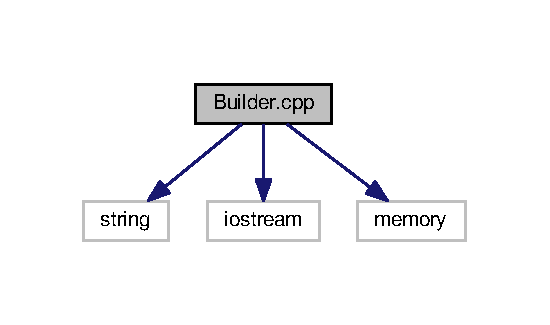
\includegraphics[width=264pt]{Builder_8cpp__incl}
\end{center}
\end{figure}
\subsection*{Classes}
\begin{DoxyCompactItemize}
\item 
class \hyperlink{classPizza}{Pizza}
\item 
class \hyperlink{classPizzaBuilder}{Pizza\+Builder}
\item 
class \hyperlink{classHawaiianPizzaBuilder}{Hawaiian\+Pizza\+Builder}
\item 
class \hyperlink{classSpicyPizzaBuilder}{Spicy\+Pizza\+Builder}
\item 
class \hyperlink{classCook}{Cook}
\end{DoxyCompactItemize}
\subsection*{Functions}
\begin{DoxyCompactItemize}
\item 
int \hyperlink{Builder_8cpp_ae66f6b31b5ad750f1fe042a706a4e3d4}{main} ()
\end{DoxyCompactItemize}


\subsection{Function Documentation}
\index{Builder.\+cpp@{Builder.\+cpp}!main@{main}}
\index{main@{main}!Builder.\+cpp@{Builder.\+cpp}}
\subsubsection[{\texorpdfstring{main()}{main()}}]{\setlength{\rightskip}{0pt plus 5cm}int main (
\begin{DoxyParamCaption}
{}
\end{DoxyParamCaption}
)}\hypertarget{Builder_8cpp_ae66f6b31b5ad750f1fe042a706a4e3d4}{}\label{Builder_8cpp_ae66f6b31b5ad750f1fe042a706a4e3d4}

\begin{DoxyCode}
116 \{
117     \hyperlink{classCook}{Cook} cook;
118     \hyperlink{classHawaiianPizzaBuilder}{HawaiianPizzaBuilder} hawaiianPizzaBuilder;
119     \hyperlink{classSpicyPizzaBuilder}{SpicyPizzaBuilder}    spicyPizzaBuilder;
120 
121     cook.\hyperlink{classCook_a14b38189b02518a8fc89c10529ea59d8}{makePizza}(&hawaiianPizzaBuilder);
122     cook.\hyperlink{classCook_a980a6342fae6617fc29fdb08101d2372}{openPizza}();
123 
124     cook.\hyperlink{classCook_a14b38189b02518a8fc89c10529ea59d8}{makePizza}(&spicyPizzaBuilder);
125     cook.\hyperlink{classCook_a980a6342fae6617fc29fdb08101d2372}{openPizza}();
126 \}\end{DoxyCode}


Here is the call graph for this function\+:\nopagebreak
\begin{figure}[H]
\begin{center}
\leavevmode
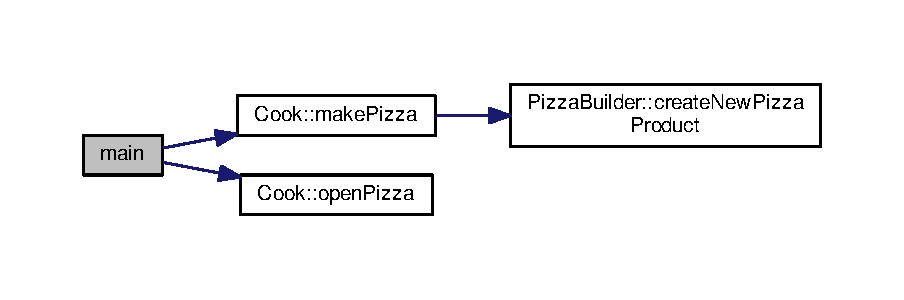
\includegraphics[width=350pt]{Builder_8cpp_ae66f6b31b5ad750f1fe042a706a4e3d4_cgraph}
\end{center}
\end{figure}



%--- End generated contents ---

% Index
\backmatter
\newpage
\phantomsection
\clearemptydoublepage
\addcontentsline{toc}{chapter}{Index}
\printindex

\end{document}
